\section{Introduction}
The system in study was proposed by O.E. R\"ossler  in 1976, as a simplified model with shape and behavior similar to spirals in Lorenz system, which was not fully understood at the time due to the techniques known to study oscillators were not applicable to Lorenz model \cite{rossler1976equation}. The R\"ossler equations are:

\begin{equation}
	\begin{array}{ll}
            \dot{x}&=-y-z\\
            \dot{y}&=x+ay\\
            \dot{z}&=b+z\left(x-c\right)
    \end{array}
\end{equation}

Although R\"ossler affirmed that the system did not have immediate physical interpretation \cite{rossler1976equation}, nowadays some applications can be found using the model as a mechanism and not as an abstraction of a physical system. The model presented has been used as a tool for image cryptography as it was shown by Mandal \textit{et al.} in  \cite{mandal2014symmetric}; in further work, Laiphrakpam and Khumanthem proposed improvements to Mandal's algorithm, as it is shown in \cite{laiphrakpam2017cryptanalysis}. On the other hand, coupled R\"ossler system with different inputs have been used to measure the correlation of time series, as Weule \textit{et al.} showed in \cite{weule1998detection}.

In order to bring the system to the real world, R\"ossler equations can be represented by a circuit, as Canals \textit{et al.} show in \cite{canals2014random}. The proposed circuit is shown in Fig. \ref{fig:circuito} and can be translated to 
\begin{equation}
	\begin{array}{ll}
            RC\dot{x}&=-y-z\\
            RC\dot{y}&=x+ay\\
            RC\dot{z}&=b+z\left(x-c\right)
    \end{array}\quad\quad\begin{array}{ll}
            a &= \dfrac{100k\Omega}{R_a}\vspace{2.5mm}\\
            b &= V_{cc}\dfrac{100k\Omega}{R_b}\vspace{2.5mm}\\
            c &= \dfrac{100k\Omega}{R_c}
    \end{array}\label{eq:circ}
\end{equation}
In \cite{canals2014random} they use this circuit to generate true random numbers using the output of the voltage of the node $z$. The nodes $x$ and $y$ have a fixed frequency of oscillation if the other variable is set to 0, since their rate of change are linear. In contrast, $z$ induces chaos to the circuit, due to its nonlinear behavior. In this manner, this variable was selected to be the output as its chaotic behavior is useful to generate random numbers \cite{canals2014random}.

In this work, the question ``for which values of input and $R_a$ a linear discrete control can successfully eliminate steady-state error ($e_{ss}$) and mitigate the overshoot in the Rössler system?''. It is believed that it will only be able to eliminate $e_{ss}$ for inputs near the operation point, since the Rössler attractor is highly sensitive to changes in the input; as for the parameters, given that PID controllers are robust, the controller will be able to work further from the operation point.

% wth 

In section \ref{sec:meth}, the dynamic system used and some theory required to design linear control systems to the Rössler equations can be found. In section \ref{sec:resultAn}, the analysis of the obtained results and their justification is made. Finally, the conclusions are presented in section \ref{sec:conc}.

%PREGUNTA INV; OBJETIVOS; TABLA CONTENIDOS, Etc.
\begin{figure*}
    \centering
    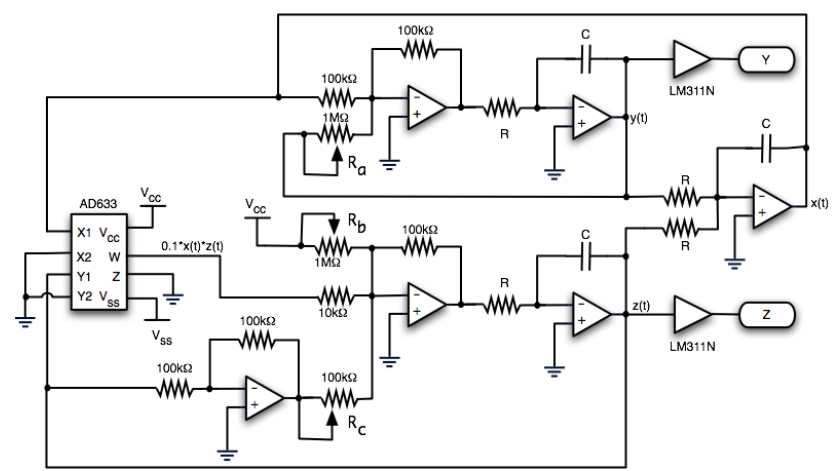
\includegraphics[scale=0.325]{files/Circuito.png}
    \caption{R\"ossler circuit representation \cite{canals2014random}.}
    \label{fig:circuito}
\end{figure*}
\section{Methods}\label{sec:meth}
\subsection{Dynamic System}
In the circuit presented, according to Canals \textit{et al.} \cite{canals2014random}, the variables $x$, $y$ and $z$ represent the voltages through the nodes shown in Fig. \ref{fig:circuito}. The $RC$ parameter defines the system's time (in seconds), the supplied voltages are $V_{cc}=15V$ and $V_{ss}=-15V$; $R_a$, $R_b$ y $R_c$ are resistors in $k\Omega$ used to calculate the system's original parameters, as shown in (\ref{eq:circ}).

The circuit can be represented through a dynamic equation, as follows:
\begin{equation}
\begin{cases}
	\dot{x_1}=\dfrac{1}{RC}\left(-x_2-x_3\right)&\vspace{2mm}\\\vspace{2mm}
	\dot{x_2}=\dfrac{1}{RC}\left(x_1+\dfrac{100k\Omega}{R_a}x_2\right)&\\
	\dot{x_3}=\dfrac{1}{RC}\left[\left(V_{cc0}+u\left(t\right)\right)\dfrac{100k\Omega}{R_b}+x_3\left(x_1-\dfrac{100k\Omega}{R_c}\right)\right]&\\
	y = x_3
\end{cases}
\label{eq:state}
\end{equation}
where $y$ is the output and $u$ the input; note that the parameter $V_{cc}$ was selected as input, based on equation (\ref{eq:circ}), thus we select an initial value $V_{cc0}$ and add the input $u\left(t\right)$ in Volts. For the rest of this document, the state variable $x_3$ can sometimes be referred as $y$, since it has been chosen as the output.

\subsection{Simulation Diagram}
Using equation system (\ref{eq:state}), a simulation diagram was constructed using \textit{Simulink}, as Fig. \ref{fig:simulink} shows.
\begin{figure}[H]
    \centering
    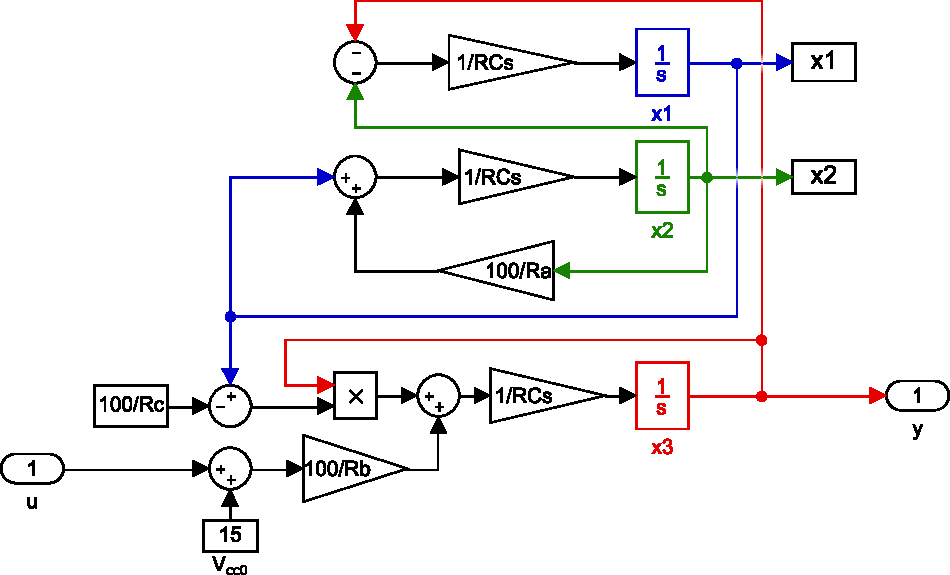
\includegraphics[scale=0.55]{files/simulink.pdf}
    \caption{Simulation diagram for R\"ossler system.}
    \label{fig:simulink}
\end{figure}

\subsection{Equilibrium Points}
The system has the following equilibrium points:
\begin{equation}
    \begin{cases}
    x_1 = \dfrac{100x_3}{R_a}&\\
    x_2 = -x_3&\\
    x_3 = \dfrac{R_a}{2R_c}\left(1\pm\sqrt{1-\dfrac{4R_c^2\left[V_{cc0}+u(t)\right]}{R_aR_b}}\right)
    \end{cases}
\end{equation}
Note the double sign in $x_3$, therefore the Rössler system has two equilibrium points. These depend on both the parameters and the input $u(t)$. In this work, the same parameters studied in \cite{JS_PL1} will be used. Thus, $R_a=500k\Omega$, $R_b=7500k\Omega$, $R_c=17.5439$, $V_{cc0}=15V$, $RC = 1$ and input
\begin{equation}\label{eq:refInput}
    u(t) = (1000V)H(t)
\end{equation}
where $H(t)$ is the Heaviside or step function. Therefore, the equilibrium points for the Rössler system with said parameters are
\begin{equation}\label{eq:operPoints}
    \begin{split}
        P_1(x_1,x_2,x_3)=(0.5228,-2.6140,2.6140)\\
        P_2(x_1,x_2,x_3)=(5.1772,-25.8859,25.8859)
    \end{split}
\end{equation}
In this paper, the first equilibrium point $P_1$ will be considered for the linearization.

\subsection{Linear Systems}
\subsubsection{Continuous}
The linearized Rössler system around $P_1$ is given by the following state space representation:
\begin{equation}\label{eq:LinearizedModel}
\begin{split}
    \Delta\mathbf{\dot{x}} =& \begin{bmatrix}
0 & -1 & -1\\
1 &0.2 & 0\\
2.614 & 0 & -5.1772
\end{bmatrix} \Delta\mathbf{x}+\begin{bmatrix}
0\\
0\\
0.0133 
\end{bmatrix}\Delta\mathbf{u}\\\vspace{5mm}
    \Delta\mathbf{y}=&\begin{bmatrix}
0 & 0 & 1
\end{bmatrix}\Delta\mathbf{x}
\end{split}
\end{equation}

 \subsubsection{Discrete}
 The discrete linear system was obtained with sample time $T=1s$, and it is presented in equation \ref{eq:discreteLinearizedModel}.
 \begin{equation}\label{eq:discreteLinearizedModel}
\begin{split}
    \Delta\mathbf{x}_{k+1} =& \begin{bmatrix}
0.245 & -0.784 & -0.0821\\
0.784 &0.743 & -0.130\\
0.215 & -0.341 & -0.0492
\end{bmatrix} \Delta\mathbf{x}_k+\begin{bmatrix}
-0.00158\\
-0.00081\\
 0.00191
\end{bmatrix}\Delta\mathbf{u}_k\\\vspace{5mm}
    \Delta\mathbf{y}_k=&\begin{bmatrix}
0 & 0 & 1
\end{bmatrix}\Delta\mathbf{x}_k
\end{split}
\end{equation}
 
\subsection{Control Requirements}
In order to design control systems, it is necessary to specify its requirements, since the control system design can vary depending on them. The requirements are often conflicting objectives. Among the wide variety of requirements for control systems, the following are some of the common ones:
\begin{itemize}
    \item Stability (relative or total).
    \item Adaptable (robust).
    \item Minimum energy consumption.
    \item Optimal behavior.
    \item Time response properties (overshoot, growth time, etc.).
    \item Precision ($e_{ss}=0$).
\end{itemize}
As it was stated, this requirements are often in conflict and they all cannot be satisfied completely, leading to a multi-objective optimization problem that tries to balance the requirements satisfied. This work will treat only with stability, precision and attempt to tweak time-response properties.

\subsection{PID Controller}
\subsubsection{Definition}
The PID controller is one of the most used scheme in industrial procedures, due to its easy tuning and usefulness in control systems in general \cite{ogata2010modern}. As its name states, the PID controller was developed on the idea of taking the proportional, integral and derivative signal of the error. Recall that the error is the difference between the reference (desired state) and the current output of the system in study:
\begin{equation}
    e(t)=r(t)-y(t)
\end{equation}
The PID continuous controller has the following transfer function:
\begin{equation}
    \dfrac{U(s)}{E(s)}=K_p\left[1+\dfrac{1}{T_is}+\dfrac{T_ds}{1+NT_ds}\right]
\end{equation}
where $N$ is a relaxation constant, $T_i$ is the integral time, $T_d$ is the derivative time and $K_p$ is the proportional gain; but in this work, the digital (discrete) PID controller will be used. Thus, the transfer function of said controller is given by
\begin{equation}
    \dfrac{U(z)}{E(z)}=\dfrac{q_0z^2+q_1z+q_2}{(z-r_1)(z-1)}.
\end{equation}
This controller has four adjustable parameters that depend on the original constants $T_i$, $T_d$, $K_p$ and $T$ (sample time). For more information on continuous and digital PID controllers, refer to \cite{discretePID}.

\subsubsection{Tuning Methods}\label{sec:tuning}
The first and more simple tuning method is almost by brute force, changing the parameters accordingly to what is desired. In the literature, the effects on the time response of each parameter are well known; in Tab. \ref{tab:pid_effects} these effects are presented. The symbol $+$ means that the parameter increases, $-$ that it decreases and $\approx$ that it does not show significant changes. The effects are shown for the growth time $t_r$, the maximum overshoot $M_p$, the settling time $t_s$ and steady-state error $e_{ss}$.

\begin{table}[ht]
\centering
\begin{tabular}{|c|cccc|}
\hline
\textbf{\backslashbox{Increment}{Effect}}             & \boldmath{$t_r$} & \boldmath{$M_p$} & \boldmath{$t_s$} & \boldmath{$e_{ss}$} \\ \hline
\boldmath{$K_p$} & -               & +               & $\approx$            & -                \\
\boldmath{$T_i$} & +               & -               & -               & +                \\
\boldmath{$T_d$} & $\approx$            & -              & -               & $\approx$            \\ \hline
\end{tabular}
\caption{Effects of the PID parameters in time response \cite{discretePID}.}
\label{tab:pid_effects}
\end{table}

The second tuning approximation is using the Zeigler-Nichols method. In this work, two variants of this method are applied: the reaction curve method and the sensitivity method.

The reaction curve method \cite{discretePID} is based on the step response of the system. This method requires a stable plant; Fig. \ref{fig:reaction_curve} illustrates how to obtain the parameters $R$ (slope) and $L$ (delay) from the tangent line at the inflection point.

\begin{figure}[H]
    \centering
    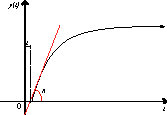
\includegraphics[scale=2.5]{files/reaction_curve.pdf}
    \caption{Reaction curve method.}
    \label{fig:reaction_curve}
\end{figure}
Based on the values for $R$ and $L$, the PID parameters can be calculated as follows:
\begin{equation}
    \begin{split}
        K_p=&\,\dfrac{1.2}{RL}\\
        T_i=&\,2L\\
        T_d=&\,0.5L
    \end{split}
\end{equation}
Although, there are many approaches to this tuning; in this work, the Chien-Hrones-Reswick rules for parameters will also be tested; the expressions to calculate the parameters are presented in Tab. \ref{tab:chien_pid}. Note that the percentages refer to the maximum overshoot of the time response.

\begin{table}[H]
\centering
\begin{tabular}{l|l}
\multicolumn{1}{c|}{\textbf{0\%}} & \multicolumn{1}{c}{\textbf{20\%}} \\ \hline
$K_p=0.95RL$                      & $K_p=\dfrac{1.2}{RL}$             \\
$T_i=2.4L$                        & $T_i=2L$                           \\
$T_d=0.42L$                       & $T_d=0.42L$                      
\end{tabular}
\caption{Chien-Hrones-Reswick rules for tuning.}
\label{tab:chien_pid}
\end{table}

Remark: for discrete systems $L=L+T/2$. The regulability (level of difficulty) of the system can be calculated: $S_0=RL$; if this value is near zero, it means that the system has a good regulability, but for values greater than 0.8 it does not \cite{discretePID}.

On the other hand, the sensitivity method \cite{discretePID} is based on the critically-stable time response, where the gain and the period of this response is used to calculate the parameters; this can be also calculated using the Bode diagram, through the gain margin and its respective frequency as follows:
\begin{equation}
    \begin{split}
        K_u =&\, 10^{\frac{M_G}{20}}\\
        T_u =&\, \dfrac{2\pi}{\omega_{cf}}
    \end{split}
\end{equation}
and then calculate the PID parameters using 
\begin{equation}
    \begin{split}
        K_p=&\,0.6K_u\\
        T_i=&\,\dfrac{T_u}{2}\\
        T_d=&\,\dfrac{T_2}{8}
    \end{split}
\end{equation}

Finally, one last analytical tuning method will be presented. Suppose you have a discrete transfer function $G(z)$ and let the discrete PID controller transfer function be $H(z)$, the closed-loop transfer function for the controlled system is
\begin{equation}
    G_{cl}(z)=\dfrac{H(z)G(z)}{1+H(z)G(z)}
\end{equation}
Therefore, the denominator of the equivalent transfer function is $P(z)=\text{Num}\{1+G(z)H(z)\}$; note that $P(z)$ is polynomial in terms of the discrete PID parameters $q_0$, $q_1$, $q_2$ and $r_1$. 

The main idea of this method is to find these PID parameters based on assigning poles to desired values and solving the system of equations for these parameters.


\subsection{Controllability Analysis}
A system is said to be controllable if there exist an unconstrained control vector that can transfer the system from an initial state $\mathbf{x}(t_0)$ to any other state in a finite interval of time \cite[p. 675]{ogata2010modern}. In order to check for controllability of a linear system, the following condition must be satisfied:
\begin{equation}
    rank\left(M_c\right)=n
\end{equation}
where $M_c$ is the controllability matrix and $n$ is the order of the system. The controllability matrix is constructed as follows:
\begin{equation}
    M_c=\begin{bmatrix}\mathbf{B}&\mathbf{AB}&\ldots&\mathbf{A}^{n-1}\mathbf{B}\end{bmatrix}
\end{equation}
For proofs of this condition and additional information, refer to \cite[pp. 675-682]{ogata2010modern}.

\subsection{Discrete Linear Feedback Controller: Pole Assignment}\label{sec:state_feed}
The idea with this controller is, using the information of all the states of a controllable system, stabilizing the output in 0 when the input reference has that same value by assigning poles. This controller is really powerful as uses more information of the system, instead of only the output as the PID controller does; on the other hand, it can only be applied in real systems when all of the states can be measured which is not always easily done. 

For a SISO linear system, if $n$ is the number of states of the system, it is done by finding a vector $\mathbf{K}_{(1 \times n)}$ such that the input of the system is given by:

\begin{equation}
    u(k) = -\mathbf{K}\mathbf{x}(k)
\end{equation}


In this manner, it can be found that the closed-loop system has the form of:

\begin{align}
    \mathbf{x}(k+1) =& \mathbf{\Phi}\mathbf{x}(k) + \mathbf{\Gamma}\mathbf{u}(k)\nonumber\\
    &\downarrow\nonumber\\
    \mathbf{x}(k+1) =& \left(\mathbf{\Phi} - \mathbf{\Gamma}\mathbf{K}\right)\mathbf{x}(k)
\end{align}

So, the poles of this closed-loop system are given by the eigenvalues of the matrix $\left(\mathbf{\Phi} - \mathbf{\Gamma}\mathbf{K}\right)$; therefore, the idea would be to find this vector that makes the matrix have some desired poles. For a SISO system, the classical method to find this vector is the Ackerman method \cite{ackermann1985multi} which is going to be used in this paper. The block model is shown in \ref{fig:feedback_ref0}.

\begin{figure}[H]
    \centering
    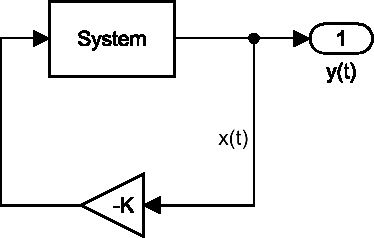
\includegraphics[scale=0.6]{files/feedback_ref0.pdf}
    \caption{Block model for a feedback controller with a reference of 0.}
    \label{fig:feedback_ref0}
\end{figure}

In \textit{MATLAB}, to use the ackerman method the function is \texttt{acker} which uses the following syntax: \texttt{$\mathbf{K}$ = acker($\mathbf{\Phi}$, $\mathbf{\Gamma}$, \textit{poles})} where \texttt{\textit{poles}} are the desired poles for the system. On the other hand, the function \texttt{place}, following the same syntax, also finds this vector with a different method but, with the restriction that the multiplicity of each pole can not be larger than the number of inputs of the system. The advantage of the second method is that it can be used when the system has different inputs.

\subsection{Discrete Linear Feedback Controller: Pole Assignment without $e_{ss}$}\label{sec:state_feed_noess}
This controller has the same purpose as the one explained above, with the difference that the input reference is not necessarily 0. In this manner, to reduce completely the $e_{ss}$ it is important to add an integrator to the plant. With this addition, the following system is obtained (for a SISO system):
\begin{align}
    \begin{bmatrix}
        \mathbf{x}(k+1) \\
        \mathbf{v}(k+1)
    \end{bmatrix}
    &= 
    \begin{bmatrix}
        \mathbf{\Phi} & \mathbf{0_{n \times 1}} \\
        \mathbf{-C} & 1
    \end{bmatrix}
    \begin{bmatrix}
        \mathbf{x}(k) \\
        \mathbf{v}(k)
    \end{bmatrix}
    +
    \begin{bmatrix}
        \mathbf{\Gamma} \\
        0
    \end{bmatrix}\mathbf{u}(k)
    +
    \begin{bmatrix}
        \mathbf{0} \\
        1
    \end{bmatrix}\mathbf{r}(k) \nonumber \\
    & \downarrow \nonumber \\
    \mathbf{\Tilde{x}}(k+1) &= \mathbf{\Tilde{\Phi}}\mathbf{\Tilde{x}}(k) + \mathbf{\Tilde{\Gamma}_1}\mathbf{u}(k) + \mathbf{\Tilde{\Gamma}_2}r(k)
\end{align}

Then, the idea is to find a vector $\mathbf{\Tilde{K}}$ such that the matrix $(\Tilde{\Phi} - \Tilde{\Gamma}_1\Tilde{K})$ has some desired poles. In this manner, using the methods explained above, we obtain the following:
\begin{equation}
    \mathbf{\Tilde{K}} = 
    \begin{bmatrix}
        \mathbf{K} & \mathbf{L}
    \end{bmatrix}
\end{equation}

The block model for this controller is shown in \ref{fig:feedback_refnot0}.
\begin{figure}[H]
    \centering
    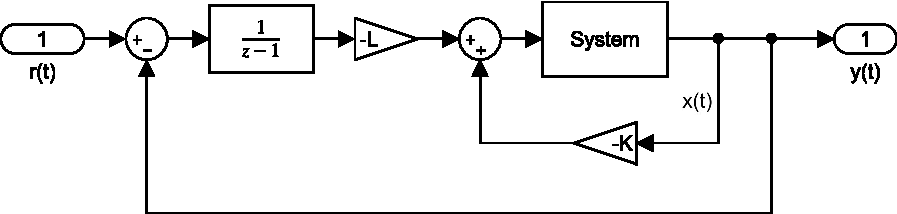
\includegraphics[scale=0.5]{files/feedback_refnot0.pdf}
    \caption{Block model for a feedback controller with an additional integrator.}
    \label{fig:feedback_refnot0}
\end{figure}
\subsection{Uncertainty Analysis}\label{sec:uncertainty}
Although there is a wide variety of uncertainty and sensitivity analysis methods, this work uses only an empirical approach to the formal uncertainty analysis. The main objective of the method here presented is to find ranges of the parameter $R_a$ where the controller behaves properly (no steady-state error and stability) for each of the controllers obtained. The idea is to change upwards and downwards $R_a$ by a $10\%$ of its initial value; based on this results, the changes can be extended in order to find ranges where the controller works or, at least, it does not saturate.

 
 
 